%%%%%%%%%%%%%%%%%%%%%%%%%%%%%%%%%%%%%%%%
\begin{figure*}[thb]
\centering
% 
\begin{subfigure}[b]{0.45\linewidth}
\centering
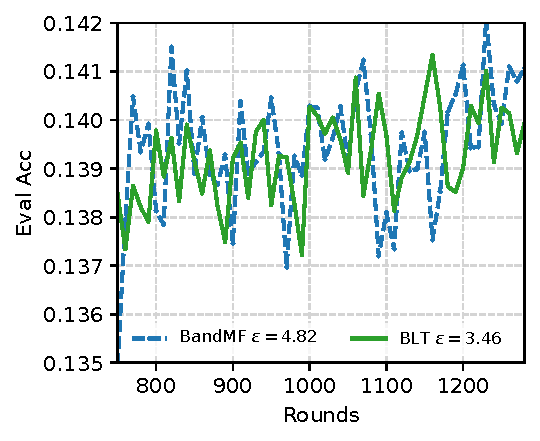
\includegraphics[width=\textwidth]{images/eses_acc2.pdf}
\caption{\small  Spanish LM in Spain (es-ES)}
\label{fig:es_acc2}
\end{subfigure}
%
\begin{subfigure}[b]{0.45\linewidth}
\centering
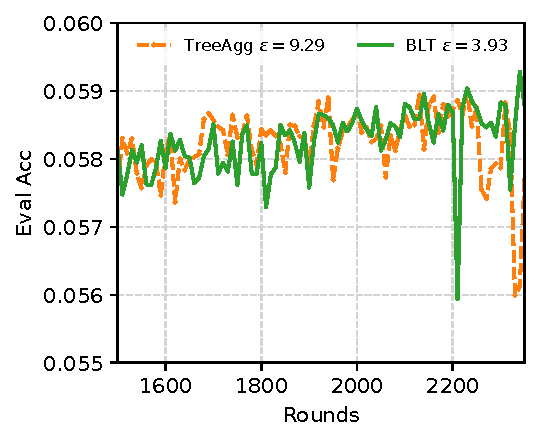
\includegraphics[width=\textwidth]{images/idid_acc2.pdf}
\caption{\small  Indonesian LM in Indonesia (id-ID)}
\label{fig:id_acc2}
\end{subfigure}
%
\begin{subfigure}[b]{0.45\linewidth}
\centering
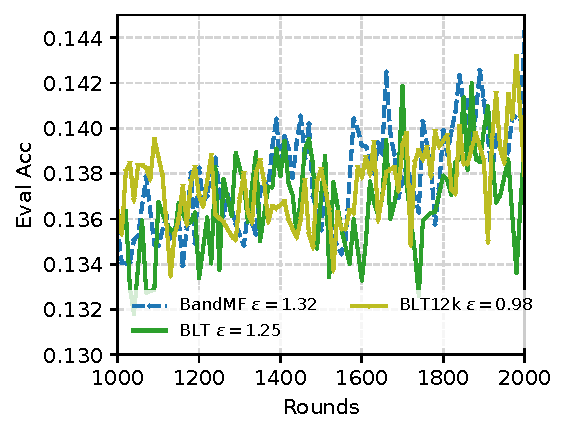
\includegraphics[width=\textwidth]{images/ptbr_acc2.pdf}
\caption{\small  Portuguese LM in Brazil (pt-BR)}
\label{fig:br_acc2}
\end{subfigure}
%
\begin{subfigure}[b]{0.45\linewidth}
\centering
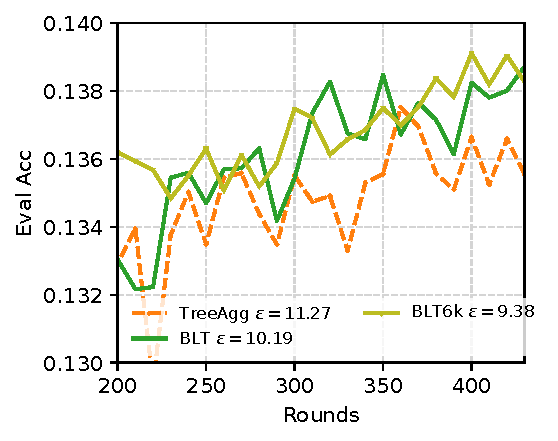
\includegraphics[width=\textwidth]{images/ptpt_acc2.pdf}
\caption{\small  Portuguese LM in Portugal (pt-PT)}
\label{fig:pt_acc2}
\end{subfigure}
%
\caption{\small  The NWP evaluation accuracy curves for training LMs with DP-FTRL in FL. Zoom in the latter stage of training for the curves in \cref{fig:acc_curve}. The NWP accuracy increases fast in the first ~200 rounds in DP FL training, and the accuracy changes within the range of $0.01$ when zooming in the later stage. The oscillation is because of the stochasticity in forming subsets of devices in both training and evaluation per round. The average NWP accuracy from nearby rounds is reported in \cref{tab:gboard} to reduce the variance. }\label{fig:acc_curve2}
\end{figure*}
%%%%%%%%%%%%%%%%%%%%%%%%%%%%%%%%%%%%%%%%